\documentclass[aspectratio=169,14pt]{beamer}
\usepackage{common}
\usepackage{memoryviz}
\usepackage{stackviz}


\title{Программирование}
\subtitle{2 | Функции}
\author{a.glushko@g.nsu.ru}
\date{14 февраля 2022}

\begin{document}

    \begin{frame}
        \titlepage
    \end{frame}

    \begin{frame}{Функции}
        \begin{itemize}
            \item $f(x) = x^2$
            \item $h(x, y) = \sqrt{x^2 + y^2}$
            \item $k! = 1 \times 2 \times \dots \times k$
            \item<2> $f: X \rightarrow Y$
        \end{itemize}
    \end{frame}

    \begin{frame}[fragile]{Функции}
        \begin{itemize}
            \item $f(x) = x^2$
            \item $f: \mathbb{N} \rightarrow \mathbb{N}$
            \item<2->
                \begin{minted}{c}
                    int f(int x) {
                        return x * x;
                    }
                \end{minted}
        \end{itemize}
    \end{frame}

    \begin{frame}[fragile]{Заголовок функции}
        \begin{center}
            \begin{tikzpicture}
                \node at (0, 2) {$\op{fun}: \mathbb{Z} \times \mathbb{R} \rightarrow \mathbb{N}$};
                \node at (0, 0)  {\code[fontsize=\normalsize]{unsigned int fun(int x, double y) }};

                \begin{onlyenv}<2->
                    \draw [decorate,decoration={brace,amplitude=5pt,raise=10pt},xshift=0pt,yshift=-4pt,color=maincolor] (-4.5, 0) -- (-1.3, 0) node[midway,yshift=0.9em] (u) {};
                    \draw [decorate,decoration={brace,amplitude=3pt,raise=10pt},xshift=0pt,yshift=-4pt,color=maincolor] (0, 0) -- (0.8, 0) node[midway,yshift=0.9em] (i) {};
                    \draw [decorate,decoration={brace,amplitude=3pt,raise=10pt},xshift=0pt,yshift=-4pt,color=maincolor] (1.8, 0) -- (3.3, 0) node[midway,yshift=0.9em] (d) {};
                    \node [yshift=-0.3em] (z) at (-0.55, 2) {};
                    \draw [->,color=maincolor] (z) to[out=-90, in=90] (i);

                    \node [yshift=-0.3em] (r) at (0.45, 2) {};
                    \draw [->,color=maincolor] (r) to[out=-90, in=90] (d);

                    \node [yshift=-0.3em] (n) at (1.6, 2) {};
                    \draw [->,color=maincolor] (n) to[out=-90, in=90] (u);
                \end{onlyenv}
            \end{tikzpicture}
        \end{center}
    \end{frame}

    \begin{frame}[fragile]{void}
        \begin{minted}{c}
            void println(int x) {
                printf("%d\n", x);
            }
        \end{minted}
    \end{frame}

    \begin{frame}[fragile]{Факториал}
        \begin{onlyenv}<1>
            \begin{minted}{c}
                int factorial(int n) {
                    // ???
                }
            \end{minted}
        \end{onlyenv}
        \begin{onlyenv}<2>
            \begin{minted}{c}
                int factorial(int n) {
                    int res = 1;
                    for (int i = 1; i < n; ++i) {
                        res *= i;
                    }
                    return res;
                }
            \end{minted}
        \end{onlyenv}
        \begin{onlyenv}<3>
            \begin{minted}{c}
                int factorial(int n) {
                    if (n == 0) {
                        return 1;
                    }
                    return n * factorial(n - 1);
                }
            \end{minted}
        \end{onlyenv}
    \end{frame}

    \begin{frame}[fragile]{Автоматическая память (стек)}
        \begin{columns}
            \begin{column}{0.5\textwidth}
                \begin{onlyenv}<-6,8->
                    \begin{minted}{c}
                        #include <stdio.h>

                        void bin(int x) {
                            int q = x / 2;
                            if (q != 0) {
                                bin(q);
                            }
                            printf("%d", x % 2);
                        }
                    \end{minted}
                \end{onlyenv}
                \begin{onlyenv}<8->
                    \vspace*{0.5\baselineskip}
                    %\hrule
                    \vspace*{0.5\baselineskip}
                    {\color{gray}OUTPUT:} \only<9->{1} \only<11->{1} \only<13->{0}
                \end{onlyenv}
                \begin{onlyenv}<7>
                    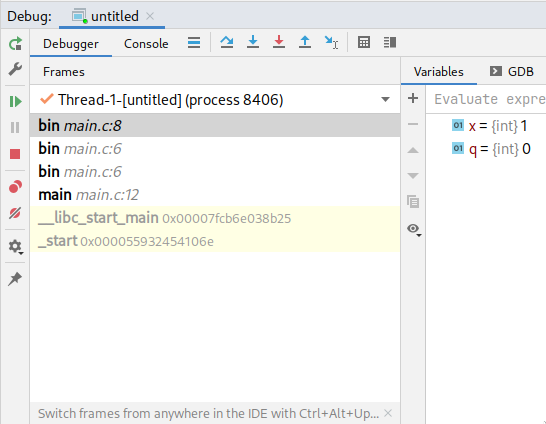
\includegraphics[width=\textwidth]{media/dbg-stack}
                \end{onlyenv}
            \end{column}
            \begin{column}{0.5\textwidth}
                \begin{onlyenv}<2>
                    \begin{itemize}
                        \item Где расположены \code{x} и \code{q}?
                    \end{itemize}
                \end{onlyenv}
                \begin{onlyenv}<3->
                    \begin{tikzpicture}[ scale=0.8 ]
                        \renewcommand{\stackright}{4}
                        \stack{8}
                        \begin{onlyenv}<4->
                            \stackframe{0}{2}{\code{bin(6)}}
                            \stackelem{0}{\code{x = 6}}
                            \stackelem{1}{\code{q = 3}}
                            \only<14->{\killframe{0}{2}}
                        \end{onlyenv}

                        \begin{onlyenv}<5->
                            \stackframe{2}{5}{\code{bin(3)}}
                            \stackelemnofill{2}{\dots}
                            \stackelem{3}{\code{x = 3}}
                            \stackelem{4}{\code{q = 1}}
                            \only<12->{\killframe{2}{5}}
                        \end{onlyenv}

                        \begin{onlyenv}<6->
                            \stackframe{5}{8}{\code{bin(1)}}
                            \stackelemnofill{5}{\dots}
                            \stackelem{6}{\code{x = 1}}
                            \stackelem{7}{\code{q = 0}}
                            \only<10->{\killframe{5}{8}}
                        \end{onlyenv}
                    \end{tikzpicture}
                \end{onlyenv}
            \end{column}
        \end{columns}
    \end{frame}

    \qnaframe

\end{document}
